\documentclass[conference]{IEEEtran}
\usepackage[utf8]{inputenc}
\usepackage[T1]{fontenc}
\usepackage[brazil]{babel}
\usepackage{amsmath,amssymb,amsfonts}
\usepackage{graphicx}
\usepackage{booktabs}
\usepackage{algorithmic}
\usepackage{textcomp}
\usepackage{xcolor}
\usepackage{url}

\graphicspath{{../results/}}

\begin{document}

\title{Análise Experimental de Sombras Volumétricas por Stencil sob Restrições Arquiteturais de Consoles Antigos}

\author{
\IEEEauthorblockN{Bruno Rafael Barbosa (RA: 112944)}
\IEEEauthorblockA{Engenharia de Computação\\
Fundação Hermínio Ometto (FHO)\\
Araras, SP, Brasil}
\and
\IEEEauthorblockN{João Pedro Magrin (RA: 113164)}
\IEEEauthorblockA{Engenharia de Computação\\
Fundação Hermínio Ometto (FHO)\\
Araras, SP, Brasil}
}

\maketitle

\begin{abstract}
Arquiteturas gráficas legadas e consoles de gerações anteriores operavam com orçamentos estritos de memória por pixel, largura reduzida de registradores nos buffers de profundidade e stencil, ausência de operações aritméticas avançadas no estágio de composição e forte limitação de taxa de preenchimento (\textit{fill rate}). Este trabalho apresenta o \textbf{Aethelion}, um ambiente experimental e rasterizador analítico em software (\texttt{cpu-sw}) projetado no contexto do Eixo~7 (Arquitetura de Consoles Antigos) para investigar quantitativamente como tais restrições arquiteturais afetam a geração de sombras volumétricas por stencil. Implementamos e validamos um instrumento de medição em conformidade integral com a Seção~4.1.5 da especificação OpenGL~1.4 (24/24 testes aprovados) e avaliamos cinco hipóteses (H1--H5) em uma cena procedural \textit{2-manifold} contra verdade de referência por \textit{ray casting} (Möller--Trumbore). Os resultados experimentais sustentam todas as hipóteses: o algoritmo \texttt{z-pass} colapsa para $F_1 = 0{,}474 \pm 0{,}175$ quando a câmera atravessa volumes de sombra (mediana de $2$ volumes contendo a câmera), enquanto \texttt{z-fail} mantém $F_1 = 1{,}000 \pm 0{,}000$; a ausência de transbordo circular (\texttt{INCR\_WRAP}/\texttt{DECR\_WRAP}) em um stencil de 3~bits gera $11.400$ saturações por quadro ($F_1 = 0{,}937$), erro eliminado ao habilitar \textit{wrap} ($F_1 = 0{,}997$); a quantização do Z-buffer para 12~bits por fragmento degrada vistas rasantes ($F_1 = 0{,}968$, revocação $0{,}944$); e a extrusão homogênea no infinito ($P_{\text{inf}}, w=0$) iguala a acurácia da extrusão finita longa ($F_1 = 0{,}9994$), superando o truncamento curto ($F_1 = 0{,}7068$).
\end{abstract}

\begin{IEEEkeywords}
Sombras volumétricas, stencil buffer, z-fail, OpenGL 1.4, arquitetura de consoles antigos, rasterização em software.
\end{IEEEkeywords}

\section{Introdução}

A evolução do hardware gráfico transformou pipelines de função fixa em arquiteturas altamente programáveis. Contudo, em consoles antigos e aceleradores gráficos de primeira geração, os recursos por pixel --- como a largura do buffer de profundidade (\textit{Z-buffer}), o número de bits do buffer de stencil, o suporte a operações modulares e a largura de banda de preenchimento --- impunham fronteiras rígidas às técnicas de sombreamento em tempo real~\cite{akenine2018}.

No contexto do Eixo~7 da disciplina de Computação Gráfica (Arquitetura de Consoles Antigos), este trabalho investiga os determinantes arquiteturais e geométricos da técnica de \textbf{sombras volumétricas por stencil} (\textit{stenciled shadow volumes}). Diferentemente de mapas de sombra (\textit{shadow maps}), que sofrem de serrilhamento por amostragem discreta, os volumes de sombra operam no espaço da tela com precisão por pixel. Entretanto, sua robustez depende diretamente de recursos específicos do pipeline gráfico: contagem fechada em stencil, aritmética de transbordo circular, precisão de profundidade e tratamento correto do plano de recorte próximo e distante~\cite{everitt2002}.

Para isolar e mensurar esses fatores de forma controlada e reprodutível, desenvolvemos o sistema \textbf{Aethelion}, um rasterizador tridimensional por software (\texttt{cpu-sw}) instrumentado com perfilamento de tempo por estágio, consumo de memória (RAM dos buffers e geometria) e comparação automatizada contra \textit{ray casting} exato. Os principais objetivos do trabalho são:
\begin{enumerate}
    \item Modelar matematicamente e implementar o pipeline completo de sombras volumétricas, incluindo a matriz de perspectiva no infinito ($P_{\text{inf}}$), extrusão homogênea ($w=0$), \textit{depth clamping} e regra de preenchimento exclusiva (\textit{top-left} orientada);
    \item Validar o instrumento de medida por meio de uma suíte de conformidade baseada na especificação OpenGL~1.4~\cite{segal2002};
    \item Avaliar experimentalmente cinco hipóteses (H1--H5) sobre custo de tampas (\texttt{z-pass} vs. \texttt{z-fail}), inversão de contagem com câmera interna, saturação versus transbordo circular no stencil, quantização de profundidade por fragmento e truncamento de extrusão, além de varreduras de resolução e complexidade geométrica.
\end{enumerate}

\section{Trabalhos Relacionados}

A formulação moderna de volumes de sombra robustos acelerados por hardware foi consolidada por Everitt e Kilgard~\cite{everitt2002}, que integraram três mecanismos para eliminar artefatos de recorte pelos planos próximo e distante: (i) posicionamento do plano distante no infinito via matriz $P_{\text{inf}}$, (ii) representação de polígonos infinitos com coordenada homogênea $w=0$, e (iii) contagem por falha no teste de profundidade (\texttt{z-fail}, ou \textit{Carmack's reverse}) com tampas frontal e traseira fechando o volume. Os autores também destacam a importância das operações de incremento e decremento com transbordo circular (\texttt{INCR\_WRAP}/\texttt{DECR\_WRAP}) para evitar saturação em cenas com alta sobreposição de volumes.

A padronização normativa dessas operações foi formalizada na especificação OpenGL~1.4 por Segal e Akeley~\cite{segal2002}, que promoveu \texttt{EXT\_stencil\_wrap} ao núcleo da API e definiu a ordem estrita de execução dos testes por fragmento (teste de stencil precedendo o teste de profundidade, Seção~4.1.5) e as regras de rasterização sem furos ou dupla cobertura (Seção~3.5).

Sob a perspectiva de avaliação experimental em tempo real e uso de recursos do padrão OpenGL~1.4, Li, Magnor e Seidel~\cite{li2003} demonstraram um sistema de reconstrução e renderização de \textit{visual hulls} em cenas reais. Embora voltado à reconstrução baseada em silhuetas de múltiplas câmeras, seu trabalho ilustra como recursos do OpenGL~1.4 reduzem o número de passagens no pipeline e como a organização experimental deve correlacionar parâmetros do algoritmo com latência, taxa de quadros e artefatos de precisão em bordas.

Do ponto de vista fundacional do pipeline gráfico, Blinn~\cite{blinn1993} formalizou a transformação de perspectiva homogênea e o recorte em espaço de clip antes da divisão por $w$, enquanto Akenine-Möller et al.~\cite{akenine2018} sintetizam a rasterização por funções de aresta e o impacto arquitetural de largura de banda e memória em GPU. O Aethelion transpõe esses conceitos para um ambiente analítico reprodutível focado em restrições de hardware legado.

\section{Metodologia e Modelagem Computacional}

\subsection{Arquitetura do Sistema e Estruturas de Dados}

O sistema foi estruturado de forma modular e componentizada em Python (\texttt{aethelion/core/}, \texttt{scenes/}, \texttt{evaluation/}, \texttt{ui/}), oferecendo três backends intercambiáveis sob um mesmo protocolo (\texttt{RendererProtocol}): rasterizador de referência em NumPy (\texttt{cpu-sw}), rasterizador acelerado via JIT Numba (\texttt{cpu-fast}) e backend de hardware em OpenGL~3.3/ModernGL (\texttt{gpu-gl}). A cena experimental consiste em uma cripta procedural composta por malhas triangulares fechadas (\textit{2-manifold}) com conectividade pré-computada: para cada malha soldada, armazenam-se vértices, índices de triângulos, arestas direcionadas (\texttt{dir\_edges}), faces incidentes (\texttt{edge\_face}) e arestas opostas (\texttt{edge\_opp}). A invariante topológica de fechamento ($\text{oposta} \ge 0$ e orientação consistente) é verificada por testes automatizados (\texttt{test\_topology.py}).

O framebuffer arquitetural simula restrições configuráveis por pixel:
\begin{itemize}
    \item \textbf{Buffer de cor}: resolução ajustável ($128\times 96$ até $3840\times 2160$), quantização de 1 a 8~bits por canal e matriz de \textit{dithering} ordenado de Bayer $4\times 4$;
    \item \textbf{Buffer de profundidade}: ponto flutuante de 32~bits (\texttt{depth\_bits=0}) ou quantizado por fragmento em $D \in \{10, 12, 16, 24\}$ bits;
    \item \textbf{Buffer de stencil} (\texttt{StencilBuffer}): largura configurável $b \in [1, 8]$ bits, modo saturado ou circular (\texttt{wrap}), e contadores observacionais de fragmentos, eventos de saturação e transbordos.
\end{itemize}

\subsection{Detecção de Silhueta e Extrusão Homogênea ($w=0$)}

Seja uma malha fechada e uma fonte de luz pontual em coordenadas homogêneas $\mathbf{L} = \langle L_x, L_y, L_z, 1 \rangle$. Uma face triangular com normal externa $\mathbf{n}_f$ e baricentro $\mathbf{c}_f$ está voltada para a luz quando:
\begin{equation}
\mathbf{n}_f \cdot (\mathbf{L} - \mathbf{c}_f) > 0.
\end{equation}
Uma aresta orientada $(v_a, v_b)$ compartilhada por duas faces adjacentes $f_1$ e $f_2$ pertence ao contorno de silhueta se, e somente se, $f_1$ está voltada para a luz e $f_2$ não está.

Para fechar o volume no infinito conforme Everitt e Kilgard~\cite{everitt2002}, cada vértice $V = \langle V_x, V_y, V_z, 1 \rangle$ das faces voltadas para a luz é extrudado como um ponto direcional com coordenada homogênea $w=0$ (normalizado pela direção unitária $\hat{\mathbf{d}} = (\mathbf{V} - \mathbf{L})/\|\mathbf{V} - \mathbf{L}\|$, o que é projetivamente invariante em $\mathbb{P}^3$ e evita estouro em \texttt{float16} ou ponto fixo):
\begin{equation}
V_\infty = \langle V_x - L_x,\; V_y - L_y,\; V_z - L_z,\; 0 \rangle \equiv \langle \hat{d}_x,\; \hat{d}_y,\; \hat{d}_z,\; 0 \rangle.
\end{equation}
Para testar a Hipótese~H5 (truncamento por extrusão curta), o sistema também suporta a extrusão finita parametrizada por comprimento $L_{\text{ext}}$:
\begin{equation}
V_{\text{fin}} = \left\langle \mathbf{V} + L_{\text{ext}} \frac{\mathbf{V} - \mathbf{L}}{\|\mathbf{V} - \mathbf{L}\|},\; 1 \right\rangle.
\end{equation}

\subsection{Matriz de Perspectiva no Infinito ($P_{\text{inf}}$) e Recorte}

Quando $w=0$, uma matriz de perspectiva com plano distante finito descartaria a tampa traseira. Tomando o limite $\text{far} \to \infty$ com folga numérica $\epsilon$~\cite{everitt2002,blinn1993}, utiliza-se:
\begin{equation}
P_{\text{inf}} =
\begin{bmatrix}
\frac{\cot(\text{fovy}/2)}{\text{aspect}} & 0 & 0 & 0 \\
0 & \cot(\text{fovy}/2) & 0 & 0 \\
0 & 0 & \epsilon - 1 & (\epsilon - 2)\,\text{near} \\
0 & 0 & -1 & 0
\end{bmatrix}.
\end{equation}
Adicionalmente, o rasterizador suporta \textit{depth clamping} (\texttt{NV\_depth\_clamp}), saturando $z_{\text{ndc}} \leftarrow \min(z_{\text{ndc}}, 1{,}0)$ nos fragmentos de volumes em \texttt{z-fail}. Antes da divisão perspectiva, o algoritmo de Sutherland--Hodgman (\texttt{clip\_near}) recorta polígonos primeiro contra o plano próximo canônico $z_{\text{clip}} + w_{\text{clip}} \ge 0$ e, em seguida, contra $w_{\text{clip}} \ge \varepsilon$.

\subsection{Regra Top-Left Orientada e Estágio de Stencil}

A rasterização exclusiva de triângulos evita furos e dupla contagem ao longo de arestas compartilhadas --- condição crítica para que o contador de stencil não acumule desvios. Seja $A$ a área assinada em espaço de tela e $s = \text{sign}(A)$. Para cada aresta $i \in \{0,1,2\}$ com função linear separável:
\begin{equation}
e_i(p_x, p_y) = s \cdot \det\begin{bmatrix} x_j - p_x & x_k - p_x \\ y_j - p_y & y_k - p_y \end{bmatrix},
\end{equation}
um centro de pixel $(p_x, p_y)$ é coberto se, e somente se, para todo $i$:
\begin{equation}
(e_i > 0) \;\lor\; \bigl(e_i = 0 \;\land\; \text{TopLeft}(s\,\Delta x_i, s\,\Delta y_i)\bigr),
\end{equation}
onde $\text{TopLeft}(dx, dy) \iff (dy < 0) \lor (dy = 0 \land dx > 0)$.

No estágio de stencil de $b \in [1, 8]$ bits com $M = 2^b - 1$, as operações saturadas e circulares seguem:
\begin{align}
\text{INCR}(s) &= \min(s + 1, M), & \text{DECR}(s) &= \max(s - 1, 0), \\
\text{INCR\_WRAP}(s) &= (s + 1) \bmod (M + 1), & \text{DECR\_WRAP}(s) &= (s - 1) \bmod (M + 1).
\end{align}
Para simular Z-buffers estreitos (Hipótese~H4), cada fragmento interpolado $z_{\text{ndc}} \in [-1, 1]$ é quantizado antes do teste de profundidade:
\begin{equation}
z_q = \frac{2}{2^D - 1}\,\text{round}\!\left(\frac{z_{\text{ndc}} + 1}{2}\,(2^D - 1)\right) - 1.
\end{equation}

O fluxo da passagem de stencil em duas sub-passagens (incremento antes de decremento para evitar \textit{underflow} espúrio em zero no modo saturado) é sintetizado abaixo:
\begin{algorithmic}[1]
\STATE \textbf{para} cada oclusor em cena \textbf{faça}
\STATE \quad Extrair arestas de silhueta e extrudar laterais (+ tampas se \texttt{z-fail})
\STATE \textbf{fim para}
\STATE Projetar triângulos de volume via $VP$ e aplicar \texttt{clip\_near}
\STATE Separar em listas $L_{\text{incr}}$ e $L_{\text{decr}}$ conforme orientação e modo (\texttt{z-pass}/\texttt{z-fail})
\STATE \textbf{para} $t \in L_{\text{incr}}$ depois $t \in L_{\text{decr}}$ \textbf{faça}
\STATE \quad Rasterizar $t$ com regra \textit{top-left}; aplicar \textit{depth clamp} e $z_q$
\STATE \quad Avaliar \texttt{dp = (z\_q < depth[y,x])} e atualizar \texttt{StencilBuffer}
\STATE \textbf{fim para}
\end{algorithmic}

\subsection{Instrumentação, Conformidade e Verdade de Referência}

Antes de qualquer coleta experimental, a suíte \texttt{conformance.py} executa 24 testes unitários cobrindo as 8 funções de comparação, 8 operações de stencil, máscaras de comparação/escrita, precedência stencil-antes-profundidade, ausência de furos/dupla cobertura na regra \textit{top-left} e recorte \texttt{clip\_near}. Todos os 24 testes obtiveram aprovação (100\%).

Para medir a acurácia objetiva das sombras, o módulo \texttt{truth.py} executa \textit{ray casting} exato (algoritmo de Möller--Trumbore) a partir das posições mundiais do G-buffer em direção à luz pontual, computando Precisão, Revocação e $F_1$-Score. O tempo gasto nessa instrumentação (e na contagem de \texttt{volumes\_with\_camera}) é isolado e descontado integralmente do cronômetro do pipeline (\texttt{ms\_total}).

\section{Resultados e Avaliação Experimental}

O roteiro experimental foi executado em modo determinístico (\texttt{--experiment --deterministic}, $\Delta t = 0{,}5\,\text{s}$, resolução base $256\times 192$, totalizando 192 quadros distribuídos em 8 fases A--H), além de três varreduras paramétricas (resolução, complexidade geométrica e regime de extrusão).

\subsection{Avaliação das Hipóteses H1--H5}

A Tabela~\ref{tab:fases} consolida os resultados das 8 fases experimentais em termos de latência mediana ($\pm$ IQR), carga geométrica, fragmentos de stencil, memória alocada e concordância ($F_1 \pm \text{DP}$). A Fig.~\ref{fig:custo} ilustra a decomposição do custo por estágio e a Fig.~\ref{fig:concordancia} compara a acurácia por fase.

\begin{table*}[t]
\centering
\caption{Resultados experimentais por fase na resolução base $256\times 192$ (backend \texttt{cpu-sw}, modo determinístico).}
\label{tab:fases}
\begin{tabular}{llccccccc}
\toprule
\textbf{Fase} & \textbf{Hip.} & \textbf{Configuração} & \textbf{ms (med. $\pm$ IQR)} & \textbf{Tris Vol.} & \textbf{Frag. Stencil} & \textbf{Mem. (KB)} & \textbf{Revoc.} & \textbf{$F_1$ ($\pm$ DP)} \\
\midrule
A — z-pass, câm. ext. & H2 & zpass, 8b, wrap, z=0, L=40 & $117{,}1 \pm 26{,}0$ & 880 & 254.054 & 571,2 & 1,000 & $0{,}999 \pm 0{,}000$ \\
B — z-fail, câm. ext. & H2 & zfail, 8b, wrap, z=0, L=40 & $172{,}2 \pm 39{,}7$ & 2.324 & 321.077 & 622,0 & 1,000 & $0{,}999 \pm 0{,}000$ \\
C — z-pass, câm. int. & H1 & zpass, 8b, wrap, z=0, L=40 & $86{,}7 \pm 9{,}1$ & 880 & 313.160 & 571,2 & 0,547 & $0{,}474 \pm 0{,}175$ \\
D — z-fail, câm. int. & H1 & zfail, 8b, wrap, z=0, L=40 & $109{,}1 \pm 14{,}1$ & 2.324 & 369.837 & 622,0 & 1,000 & $1{,}000 \pm 0{,}000$ \\
E — 3b sem wrap       & H3 & zfail, 3b, sat., z=0, L=40 & $95{,}9 \pm 16{,}8$ & 2.340 & 573.014 & 592,5 & 0,889 & $0{,}937 \pm 0{,}036$ \\
F — 3b com wrap       & H3 & zfail, 3b, wrap, z=0, L=40 & $105{,}8 \pm 33{,}8$ & 2.340 & 573.014 & 592,5 & 1,000 & $0{,}997 \pm 0{,}001$ \\
G — depth 12 bits     & H4 & zfail, 8b, wrap, z=12, L=40 & $150{,}1 \pm 12{,}7$ & 2.316 & 315.366 & 501,7 & 0,944 & $0{,}968 \pm 0{,}028$ \\
H — extrusão curta    & H5 & zfail, 8b, wrap, z=0, L=3.5 & $159{,}4 \pm 27{,}9$ & 2.324 & 217.841 & 622,0 & 0,763 & $0{,}857 \pm 0{,}105$ \\
\bottomrule
\end{tabular}
\end{table*}

\begin{figure}[t]
\centering
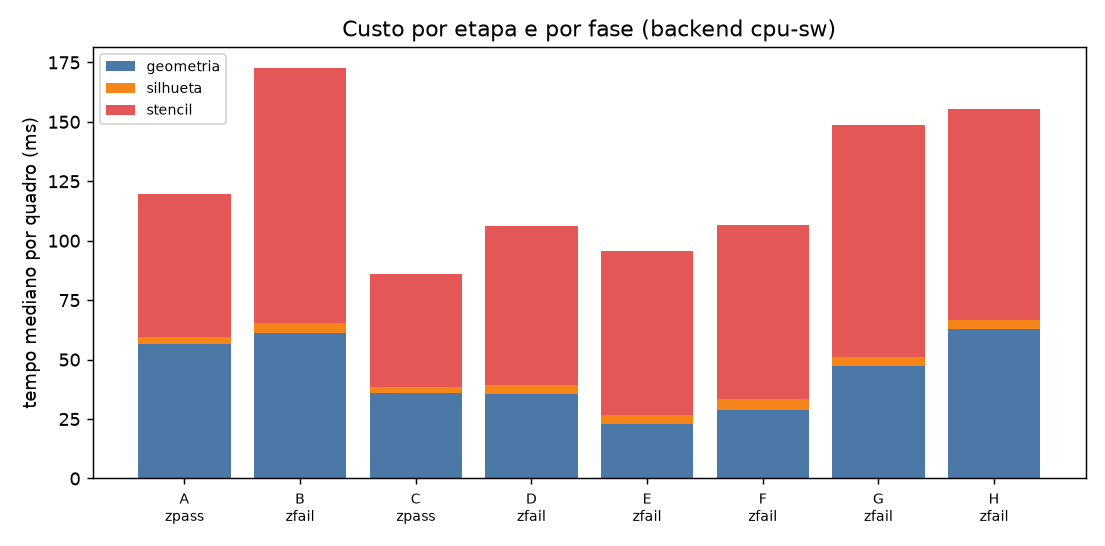
\includegraphics[width=\columnwidth]{grafico_custo_etapas.png}
\caption{Tempo mediano por estágio do pipeline (geometria, silhueta e stencil) nas 8 fases experimentais.}
\label{fig:custo}
\end{figure}

\begin{figure}[t]
\centering
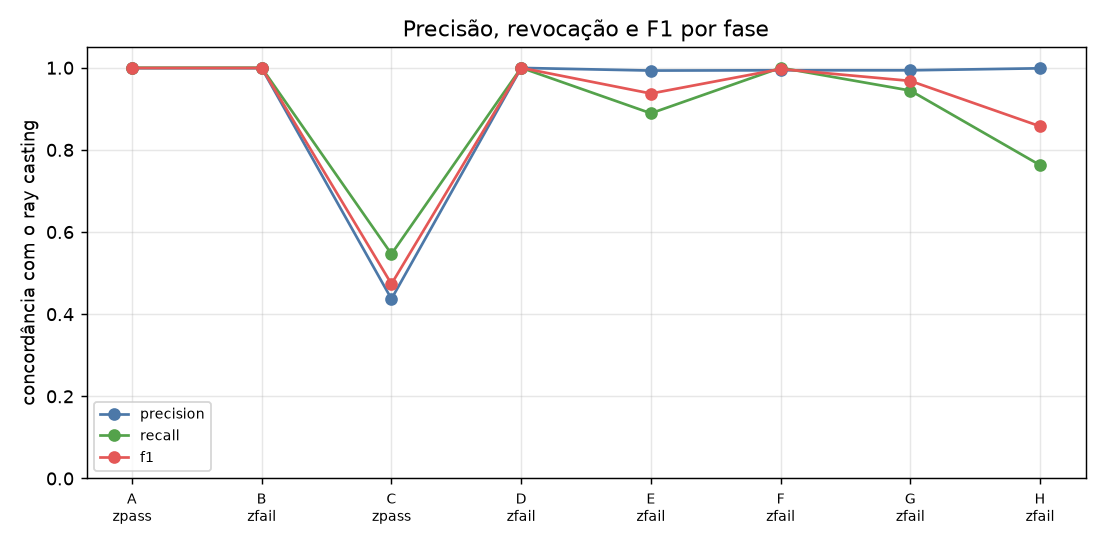
\includegraphics[width=\columnwidth]{grafico_concordancia.png}
\caption{Precisão, revocação e $F_1$-Score contra a verdade de referência por \textit{ray casting} em cada fase.}
\label{fig:concordancia}
\end{figure}

Os dados sustentam integralmente as cinco hipóteses formuladas:
\begin{itemize}
    \item \textbf{H1 (C vs. D — Sustentada):} Na trajetória com câmera externa (A vs. B), \texttt{z-pass} ($F_1=0{,}999$) e \texttt{z-fail} ($F_1=0{,}999$) concordam integralmente. Quando a câmera atravessa os volumes (Fase~C, mediana de $2$ volumes contendo a câmera), o recorte pelo plano próximo corrompe a contagem de \texttt{z-pass}, derrubando o desempenho para $F_1 = 0{,}474 \pm 0{,}175$, enquanto \texttt{z-fail} (Fase~D) preserva $F_1 = 1{,}000 \pm 0{,}000$.
    \item \textbf{H2 (A vs. B — Sustentada):} O processamento das tampas frontal e traseira em \texttt{z-fail} eleva a carga geométrica de 880 para 2.324 triângulos de volume (+164,1\%) e a latência mediana de $117{,}1\,\text{ms}$ para $172{,}2\,\text{ms}$ (+47,1\%), além de aumentar o consumo de memória de $571{,}2\,\text{KB}$ para $622{,}0\,\text{KB}$.
    \item \textbf{H3 (E vs. F — Sustentada):} Em um buffer de stencil estreito de 3~bits ($M=7$) sob alta sobreposição ($573.014$ fragmentos de stencil idênticos em E e F), as operações saturadas (\texttt{INCR}/\texttt{DECR}) registram $11.400$ eventos de saturação por quadro (mediana), degradando a revocação para $0{,}889$ ($F_1 = 0{,}937$). A habilitação de \texttt{INCR\_WRAP}/\texttt{DECR\_WRAP} converte as saturações em $6.836$ transbordos circulares válidos e restaura a acurácia para $F_1 = 0{,}997$ (revocação $1{,}000$), conforme mostrado na Fig.~\ref{fig:stencil}.
    \item \textbf{H4 (G vs. B — Sustentada):} Reduzir a precisão do Z-buffer para 12~bits por fragmento em vistas rasantes economiza memória nos buffers ($501{,}7\,\text{KB}$ contra $622{,}0\,\text{KB}$), mas introduz colisões de profundidade (\textit{z-fighting}) entre geometria e volumes, reduzindo a revocação para $0{,}944$ ($F_1 = 0{,}968$).
    \item \textbf{H5 (H vs. B — Sustentada):} Truncar a extrusão finita em $L = 3{,}5$ reduz a revocação para $0{,}763$ ($F_1 = 0{,}857 \pm 0{,}105$), pois os volumes deixam de alcançar receptores distantes.
\end{itemize}

\begin{figure}[t]
\centering
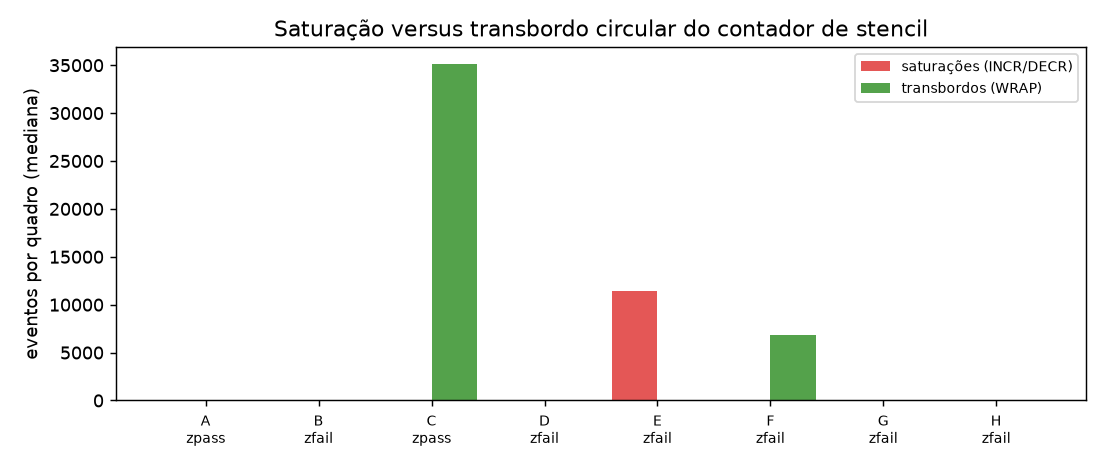
\includegraphics[width=\columnwidth]{grafico_stencil.png}
\caption{Eventos de saturação (Fase E) versus transbordos circulares válidos (Fase F) em stencil de 3~bits.}
\label{fig:stencil}
\end{figure}

\subsection{Varreduras Paramétricas: Resolução, Complexidade e $P_{\text{inf}}$}

As Tabelas~\ref{tab:res}, \ref{tab:det} e \ref{tab:ext} e as Figs.~\ref{fig:var_res}--\ref{fig:var_ext} apresentam os resultados das varreduras paramétricas em \texttt{z-fail} (8~bits, \textit{wrap} ativo).

\begin{table}[t]
\centering
\caption{Varredura de resolução interna (\texttt{z-fail}, 8~bits).}
\label{tab:res}
\begin{tabular}{lcccc}
\toprule
\textbf{Resolução} & \textbf{ms (med. $\pm$ IQR)} & \textbf{FPS} & \textbf{Mem. (KB)} & \textbf{$F_1$} \\
\midrule
$160\times 120$ & $154{,}1 \pm 24{,}0$ & 6,49 & 387,6 & 0,9996 \\
$256\times 192$ & $197{,}8 \pm 23{,}0$ & 5,06 & 621,6 & 0,9994 \\
$320\times 240$ & $241{,}6 \pm 47{,}7$ & 4,15 & 837,6 & 0,9994 \\
$400\times 300$ & $242{,}2 \pm 28{,}9$ & 4,13 & 1.175,1 & 0,9996 \\
\bottomrule
\end{tabular}
\end{table}

\begin{table}[t]
\centering
\caption{Varredura de complexidade geométrica (\texttt{detail}, $256\times 192$).}
\label{tab:det}
\begin{tabular}{lcccc}
\toprule
\textbf{Complexidade} & \textbf{Tris Cena / Vol.} & \textbf{ms (med. $\pm$ IQR)} & \textbf{Mem. (KB)} & \textbf{$F_1$} \\
\midrule
\texttt{detail=0.5} & 876 / 1.472 & $130{,}6 \pm 39{,}4$ & 545,3 & 0,9996 \\
\texttt{detail=1.0} & 1.540 / 2.312 & $179{,}9 \pm 23{,}7$ & 621,6 & 0,9994 \\
\texttt{detail=1.5} & 2.424 / 3.368 & $229{,}5 \pm 21{,}4$ & 720,8 & 0,9996 \\
\texttt{detail=2.0} & 3.680 / 4.768 & $304{,}7 \pm 31{,}5$ & 858,4 & 0,9997 \\
\bottomrule
\end{tabular}
\end{table}

\begin{table}[t]
\centering
\caption{Comparação entre extrusão finita e homogênea no infinito ($P_{\text{inf}}, w=0$).}
\label{tab:ext}
\begin{tabular}{lcccc}
\toprule
\textbf{Regime de Extrusão} & \textbf{Precisão} & \textbf{Revocação} & \textbf{$F_1$} & \textbf{ms (med.)} \\
\midrule
Finita curta ($L=3{,}5$) & 0,9981 & 0,5497 & 0,7068 & 162,1 \\
Finita padrão ($L=40$)  & 0,9990 & 0,9999 & 0,9994 & 174,8 \\
Infinita $P_{\text{inf}}$ ($w=0$) & 0,9990 & 0,9999 & 0,9994 & 183,0 \\
\bottomrule
\end{tabular}
\end{table}

Na varredura de resolução (Tabela~\ref{tab:res}), o consumo de memória cresce linearmente com o número de pixels (de $387{,}6\,\text{KB}$ para $1.175{,}1\,\text{KB}$), mantendo $F_1 > 0{,}999$ em todas as escalas, enquanto a latência mediana cresce monotonicamente de $154{,}1\,\text{ms}$ ($160\times 120$) até $242{,}2\,\text{ms}$ ($400\times 300$, com $9{,}47\times 10^5$ fragmentos de stencil). Na varredura de complexidade (Tabela~\ref{tab:det}), quadruplicar a densidade geométrica eleva os triângulos de volume de $1.472$ para $4.768$ e o tempo de $130{,}6\,\text{ms}$ para $304{,}7\,\text{ms}$. Por fim, a extrusão homogênea no infinito ($P_{\text{inf}}, w=0$, Tabela~\ref{tab:ext}) atinge $F_1 = 0{,}9994$ (revocação $0{,}9999$), igualando a extrusão finita longa sem depender de um parâmetro heurístico de alcance máximo.

\begin{figure}[t]
\centering
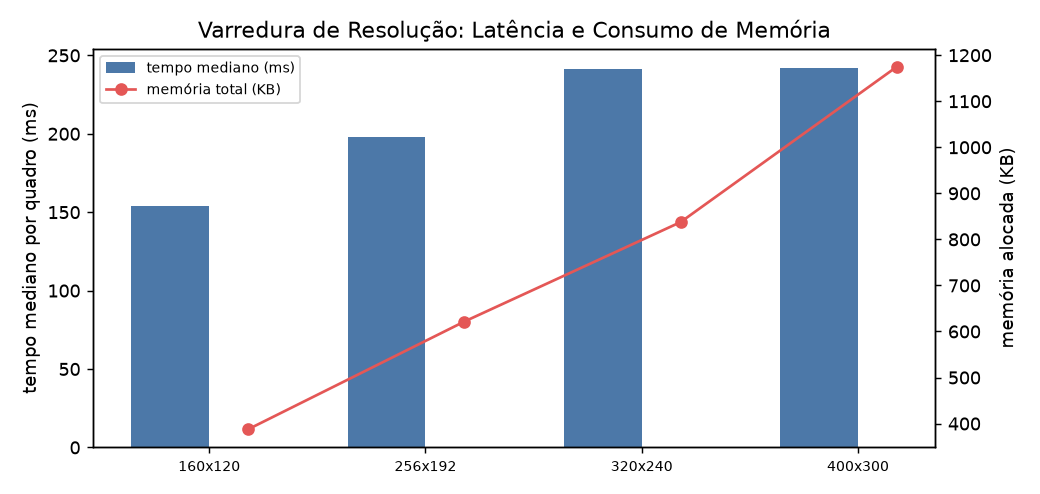
\includegraphics[width=\columnwidth]{grafico_varredura_resolucao.png}
\caption{Varredura de resolução interna: tempo mediano por quadro e consumo total de memória.}
\label{fig:var_res}
\end{figure}

\begin{figure}[t]
\centering
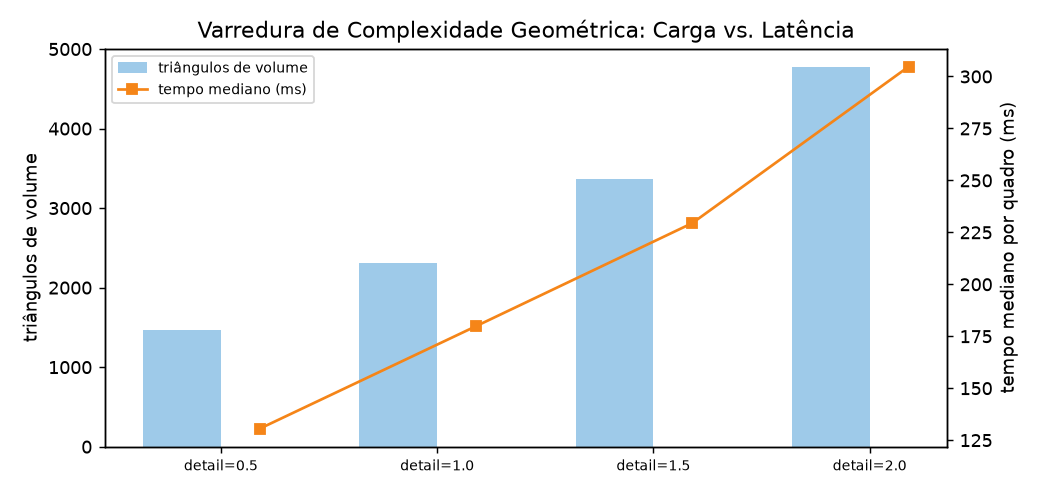
\includegraphics[width=\columnwidth]{grafico_varredura_complexidade.png}
\caption{Varredura de complexidade geométrica: crescimento de triângulos de volume versus latência.}
\label{fig:var_det}
\end{figure}

\begin{figure}[t]
\centering
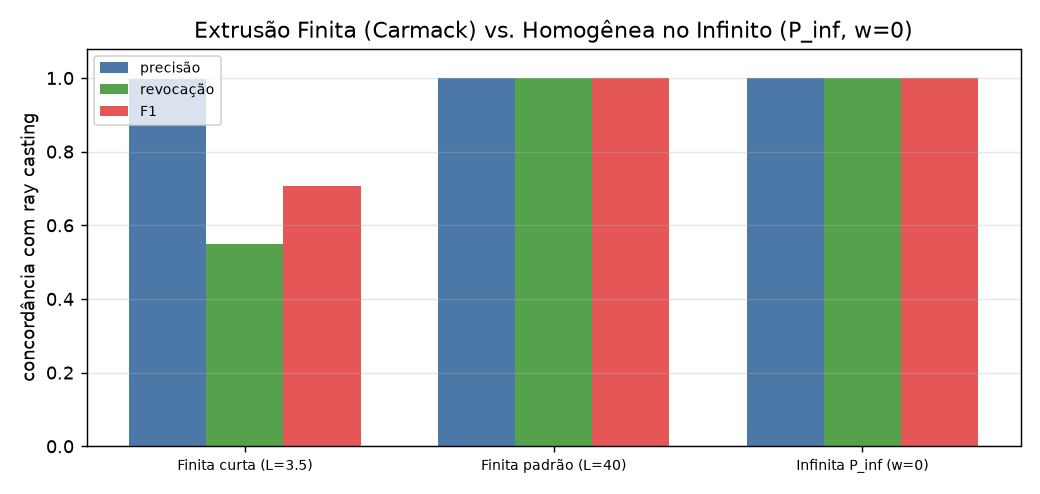
\includegraphics[width=\columnwidth]{grafico_varredura_extrusao.png}
\caption{Comparação de precisão, revocação e $F_1$ entre extrusão finita curta, padrão e infinita ($P_{\text{inf}}, w=0$).}
\label{fig:var_ext}
\end{figure}

\section{Conclusão, Limitações e Trabalhos Futuros}

Este trabalho demonstrou, por meio de um rasterizador validado em conformidade com o OpenGL~1.4, como limitações arquiteturais típicas de consoles antigos condicionam a qualidade e o custo das sombras volumétricas por stencil. Todas as cinco hipóteses experimentais (H1--H5) foram sustentadas pelos dados, evidenciando a necessidade conjunta do algoritmo \texttt{z-fail}, de operações circulares \texttt{INCR\_WRAP}/\texttt{DECR\_WRAP}, de precisão adequada no Z-buffer e de extrusão suficiente ou homogênea no infinito ($P_{\text{inf}}, w=0$).

Como limitações declaradas do instrumento: (i) no backend analítico em software (\texttt{cpu-sw}), os tempos absolutos ($\approx 4$--$6{,}5\,\text{FPS}$ em $256\times 192$) refletem o despacho por triângulo em CPU e servem para comparações relativas entre fases (enquanto os backends \texttt{cpu-fast} e \texttt{gpu-gl} aceleram a exploração interativa); e (ii) na ausência de rasterização homogênea 4D sem divisão perspectiva, quando vértices da tampa traseira no infinito ($w_e=0$, onde $z_{\text{clip}}=w_{\text{clip}}$ sob $P_{\text{inf}}$) apontam para trás da câmera ($w_{\text{clip}} \le 10^{-3}$), o sistema ancora a extrusão em distância finita longa ($L=500$) para evitar singularidade de $w_{\text{clip}}=0$ no recorte próximo. Como trabalhos futuros, planeja-se explorar extrusão de silhuetas diretamente em \textit{geometry/compute shaders} na GPU, múltiplas fontes de luz com atenuação penumbral e técnicas de descarte (\textit{scissor/depth bounds culling}) de volumes para reduzir o consumo de \textit{fill rate}.

\begin{thebibliography}{1}

\bibitem{everitt2002}
C.~Everitt e M.~J. Kilgard, ``Practical and robust stenciled shadow volumes for hardware-accelerated rendering,'' NVIDIA Corporation, Tech. Rep., 2002. [Online]. Available: \url{https://arxiv.org/abs/cs/0301002}

\bibitem{segal2002}
M.~Segal e K.~Akeley, \emph{The OpenGL Graphics System: A Specification (Version 1.4)}. Silicon Graphics, Inc., 2002.

\bibitem{li2003}
M.~Li, M.~Magnor, e H.-P. Seidel, ``Online accelerated rendering of visual hulls in real scenes,'' \emph{Journal of WSCG}, vol.~11, no.~1, pp. 290--297, 2003.

\bibitem{akenine2018}
T.~Akenine-Möller, E.~Haines, e N.~Hoffman, \emph{Real-Time Rendering}, 4th~ed. Boca Raton, FL, USA: CRC Press, 2018.

\bibitem{blinn1993}
J.~F. Blinn, ``A trip down the graphics pipeline: The homogeneous perspective transform,'' \emph{IEEE Computer Graphics and Applications}, vol.~13, no.~3, pp. 75--80, 1993.

\end{thebibliography}

\end{document}
